\section{Theory}
\label{sec:theory}

\subsection{Interference of Coherent Light}
\label{sec:interference}
Interference is a phenomenon where two waves superpose to form a resultant wave. 
This typically occurs when waves of compatible frequencies and phases converge, 
resulting in constructive or destructive interference patterns. 
A crucial requirement for observing clear interference patterns is \textit{coherence}.

Coherence refers to a consistent phase relationship between the waves. 
It is distinguished into temporal and spatial coherence. Temporal coherence 
relates to the duration over which a wave's phase and amplitude remain predictable. 
Spatial coherence, on the other hand, refers to the uniformity of the light wave's 
phase across different areas of the wavefront. 
A laser beam, owing to its production process, exhibits high temporal and spatial 
coherence. The degree of coherence can be quantified as
\begin{equation}
    \gamma_{1,2}(\vec{r}_1,t_1;\vec{r}_2,t_2)=
    \frac{\langle E(\vec{r}_1,t_1)E^*(\vec{r}_2,t_2) \rangle}{\sqrt{\langle |E(\vec{r}_1,t_1)|^2 \rangle\langle |E(\vec{r}_2,t_2)|^2 \rangle}}
    \label{eqn:degree}
\end{equation}
where $E(\vec{r}_i,t_i)$ represents the amplitude of the electric field at position $\vec{r}_i$ 
and time $t_i$. A $\gamma_{1,2}$ value of \num{0} indicates complete incoherence, while 
\num{1} signifies perfect coherence.

Electromagnetic waves are transverse oscillations in the electromagnetic field, 
exhibiting different polarizations depending on their oscillation direction. 
Light can be polarized by passing through a polarization filter. Unpolarized light 
comprises multiple polarizations in various directions. A polarization filter 
allows only a specific polarization to pass through, effectively filtering out a 
single polarization from the unpolarized beam.

An alternative method for obtaining polarized light involves the use of a polarizing 
beam splitter cube (PBSC). This cube differentiates between s-polarized and 
p-polarized light: it reflects the s-polarized light, which oscillates perpendicular 
to the plane, and transmits the p-polarized light, oscillating parallel to the plane.

\begin{figure}
    \centering
    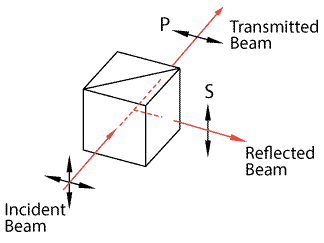
\includegraphics[width=0.4\textwidth]{pictures/PBSC.png}
    \caption{Schematic illustration of a Polarizing Beam Splitter Cube (PBSC). The cube divides an incident unpolarized beam into two components: one s-polarized and one p-polarized. \cite{PBSC}}
    \label{fig:PBSC}
\end{figure}

While the degree of coherence, as defined in Equation \eqref{eqn:degree}, is a reliable 
measure for describing coherence, assessing the contrast of the interference pattern 
offers a more practical approach. The contrast, denoted by $K$, is defined as
\begin{equation}
    K=\frac{I_\text{max}-I_\text{min}}{I_\text{max}+I_\text{min}},
    \label{eqn:contrast}
\end{equation}
where $I_\text{max}$ and $I_\text{min}$ are the maximum and minimum intensities in the 
interference pattern. Analogous to the degree of coherence, $K$ ranges from 
\numrange{0}{1}, with a perfect contrast represented by $K=1$.

Since the intensity $I$ is proportional to the superposition of two waves, expressed as
\begin{equation*}
    I\propto \langle |E_1\cos(\omega t)+E_2\cos(\omega t +\delta)|^2 \rangle
    \label{eqn:intensity}
\end{equation*}
where $\omega$ is the wave frequency and $\delta$ represents the phase difference 
between the two waves. Consequently, the maximal and minimal intensities can be written as
\begin{align*}
    I_\text{max/min}\propto\frac{1}{2}(E_1^2+E_2^2)\pm E_1E_2.
\end{align*}
The electric field depends on the polarization angle $\phi$ of the incoming beam, given by
\begin{align*}
    E_1&=\sqrt{E_1+E_2}\cos(\phi) \\
    E_2&=\sqrt{E_1+E_2}\sin(\phi).
\end{align*}
Substituting these into the intensity equation \eqref{eqn:intensity} yields
\begin{equation*}
    I_\text{max/min}\propto (1\pm 2\sin(\phi)\cos(\phi)).
\end{equation*}
Therefore, the contrast $K$, as defined in Equation \eqref{eqn:contrast}, can be 
expressed as a function of the initial polarization angle $\phi$:
\begin{equation}
    K=2|\sin(\phi)\cos(\phi)|
    \label{eqn:contrast2}
\end{equation}

\subsection{Refraction Indices of Glass and Gases}
The refractive index, denoted as $n$, characterizes how the speed of light in a medium $v$ 
compares to its speed in a vacuum $c$. Mathematically, it is expressed as
\begin{equation*}
    n=\frac{v}{c}.
\end{equation*}
Due to the change in light speed upon entering a medium with a different refractive index, 
a path length difference arises for a beam traversing through such a medium. 
When two waves with a phase difference $\Delta\Phi$ interfere, the number of intensity 
maxima and minima, $M$, is calculated as
\begin{equation}
    M=\frac{\Delta\Phi}{2\pi}
    \label{eqn:M}
\end{equation}
For glass, this phase difference is determined by
\begin{equation}
    \Delta\Phi(\theta)=2\pi\frac{T}{\lambda_\text{vac}}\frac{n-1}{2n}\theta^2
    \label{eqn:delta1}
\end{equation}
where $T$ is the glass thickness, $\lambda_\text{vac}$ is the wavelength in vacuum, and $\theta$ 
is the angle of incidence. For glass plates pre-tilted at angles $\theta_1$ and $\theta_2$, 
the equation \eqref{eqn:delta1} modifies to
\begin{equation}
    \Delta\Phi(\theta)=2\pi\frac{T}{\lambda_\text{vac}}\frac{n-1}{n}[(\theta+\theta_1)^2-(\theta+\theta_2)^2].
    \label{eqn:delta}
\end{equation}

Similar to Equation \eqref{eqn:delta1}, the phase difference for a gas is represented by
\begin{equation*}
    \Delta\Phi=2\pi\frac{T}{\lambda_\text{vac}}(n-1).
\end{equation*}
Additionally, the refractive index of an ideal gas can be approximated using the Lorentz-Lorenz law, 
which relates it to the gas's pressure $p$ and temperature $T$. The Lorentz-Lorenz formula is expressed as
\begin{equation}
    \frac{n^2-1}{n^2+1}=\frac{Ap}{RT}
    \label{eqn:LLL}
\end{equation}
where $R$ denotes the universal gas constant and $A$ represents the molecular refractivity of the gas.
